\documentclass[]{article}
\usepackage{lmodern}
\usepackage{amssymb,amsmath}
\usepackage{ifxetex,ifluatex}
\usepackage{fixltx2e} % provides \textsubscript
\ifnum 0\ifxetex 1\fi\ifluatex 1\fi=0 % if pdftex
  \usepackage[T1]{fontenc}
  \usepackage[utf8]{inputenc}
\else % if luatex or xelatex
  \ifxetex
    \usepackage{mathspec}
  \else
    \usepackage{fontspec}
  \fi
  \defaultfontfeatures{Ligatures=TeX,Scale=MatchLowercase}
\fi
% use upquote if available, for straight quotes in verbatim environments
\IfFileExists{upquote.sty}{\usepackage{upquote}}{}
% use microtype if available
\IfFileExists{microtype.sty}{%
\usepackage{microtype}
\UseMicrotypeSet[protrusion]{basicmath} % disable protrusion for tt fonts
}{}
\usepackage[margin=1in]{geometry}
\usepackage{hyperref}
\hypersetup{unicode=true,
            pdftitle={Laborator 5},
            pdfborder={0 0 0},
            breaklinks=true}
\urlstyle{same}  % don't use monospace font for urls
\usepackage{color}
\usepackage{fancyvrb}
\newcommand{\VerbBar}{|}
\newcommand{\VERB}{\Verb[commandchars=\\\{\}]}
\DefineVerbatimEnvironment{Highlighting}{Verbatim}{commandchars=\\\{\}}
% Add ',fontsize=\small' for more characters per line
\usepackage{framed}
\definecolor{shadecolor}{RGB}{248,248,248}
\newenvironment{Shaded}{\begin{snugshade}}{\end{snugshade}}
\newcommand{\KeywordTok}[1]{\textcolor[rgb]{0.13,0.29,0.53}{\textbf{#1}}}
\newcommand{\DataTypeTok}[1]{\textcolor[rgb]{0.13,0.29,0.53}{#1}}
\newcommand{\DecValTok}[1]{\textcolor[rgb]{0.00,0.00,0.81}{#1}}
\newcommand{\BaseNTok}[1]{\textcolor[rgb]{0.00,0.00,0.81}{#1}}
\newcommand{\FloatTok}[1]{\textcolor[rgb]{0.00,0.00,0.81}{#1}}
\newcommand{\ConstantTok}[1]{\textcolor[rgb]{0.00,0.00,0.00}{#1}}
\newcommand{\CharTok}[1]{\textcolor[rgb]{0.31,0.60,0.02}{#1}}
\newcommand{\SpecialCharTok}[1]{\textcolor[rgb]{0.00,0.00,0.00}{#1}}
\newcommand{\StringTok}[1]{\textcolor[rgb]{0.31,0.60,0.02}{#1}}
\newcommand{\VerbatimStringTok}[1]{\textcolor[rgb]{0.31,0.60,0.02}{#1}}
\newcommand{\SpecialStringTok}[1]{\textcolor[rgb]{0.31,0.60,0.02}{#1}}
\newcommand{\ImportTok}[1]{#1}
\newcommand{\CommentTok}[1]{\textcolor[rgb]{0.56,0.35,0.01}{\textit{#1}}}
\newcommand{\DocumentationTok}[1]{\textcolor[rgb]{0.56,0.35,0.01}{\textbf{\textit{#1}}}}
\newcommand{\AnnotationTok}[1]{\textcolor[rgb]{0.56,0.35,0.01}{\textbf{\textit{#1}}}}
\newcommand{\CommentVarTok}[1]{\textcolor[rgb]{0.56,0.35,0.01}{\textbf{\textit{#1}}}}
\newcommand{\OtherTok}[1]{\textcolor[rgb]{0.56,0.35,0.01}{#1}}
\newcommand{\FunctionTok}[1]{\textcolor[rgb]{0.00,0.00,0.00}{#1}}
\newcommand{\VariableTok}[1]{\textcolor[rgb]{0.00,0.00,0.00}{#1}}
\newcommand{\ControlFlowTok}[1]{\textcolor[rgb]{0.13,0.29,0.53}{\textbf{#1}}}
\newcommand{\OperatorTok}[1]{\textcolor[rgb]{0.81,0.36,0.00}{\textbf{#1}}}
\newcommand{\BuiltInTok}[1]{#1}
\newcommand{\ExtensionTok}[1]{#1}
\newcommand{\PreprocessorTok}[1]{\textcolor[rgb]{0.56,0.35,0.01}{\textit{#1}}}
\newcommand{\AttributeTok}[1]{\textcolor[rgb]{0.77,0.63,0.00}{#1}}
\newcommand{\RegionMarkerTok}[1]{#1}
\newcommand{\InformationTok}[1]{\textcolor[rgb]{0.56,0.35,0.01}{\textbf{\textit{#1}}}}
\newcommand{\WarningTok}[1]{\textcolor[rgb]{0.56,0.35,0.01}{\textbf{\textit{#1}}}}
\newcommand{\AlertTok}[1]{\textcolor[rgb]{0.94,0.16,0.16}{#1}}
\newcommand{\ErrorTok}[1]{\textcolor[rgb]{0.64,0.00,0.00}{\textbf{#1}}}
\newcommand{\NormalTok}[1]{#1}
\usepackage{graphicx,grffile}
\makeatletter
\def\maxwidth{\ifdim\Gin@nat@width>\linewidth\linewidth\else\Gin@nat@width\fi}
\def\maxheight{\ifdim\Gin@nat@height>\textheight\textheight\else\Gin@nat@height\fi}
\makeatother
% Scale images if necessary, so that they will not overflow the page
% margins by default, and it is still possible to overwrite the defaults
% using explicit options in \includegraphics[width, height, ...]{}
\setkeys{Gin}{width=\maxwidth,height=\maxheight,keepaspectratio}
\IfFileExists{parskip.sty}{%
\usepackage{parskip}
}{% else
\setlength{\parindent}{0pt}
\setlength{\parskip}{6pt plus 2pt minus 1pt}
}
\setlength{\emergencystretch}{3em}  % prevent overfull lines
\providecommand{\tightlist}{%
  \setlength{\itemsep}{0pt}\setlength{\parskip}{0pt}}
\setcounter{secnumdepth}{5}
% Redefines (sub)paragraphs to behave more like sections
\ifx\paragraph\undefined\else
\let\oldparagraph\paragraph
\renewcommand{\paragraph}[1]{\oldparagraph{#1}\mbox{}}
\fi
\ifx\subparagraph\undefined\else
\let\oldsubparagraph\subparagraph
\renewcommand{\subparagraph}[1]{\oldsubparagraph{#1}\mbox{}}
\fi

%%% Use protect on footnotes to avoid problems with footnotes in titles
\let\rmarkdownfootnote\footnote%
\def\footnote{\protect\rmarkdownfootnote}

%%% Change title format to be more compact
\usepackage{titling}

% Create subtitle command for use in maketitle
\newcommand{\subtitle}[1]{
  \posttitle{
    \begin{center}\large#1\end{center}
    }
}

\setlength{\droptitle}{-2em}

  \title{Laborator 5}
    \pretitle{\vspace{\droptitle}\centering\huge}
  \posttitle{\par}
  \subtitle{Exemple de algoritmi randomizați}
  \author{}
    \preauthor{}\postauthor{}
    \date{}
    \predate{}\postdate{}
  
\usepackage{booktabs}
\usepackage{longtable}
\usepackage{framed,color}
\definecolor{shadecolor}{RGB}{248, 248, 248}
\definecolor{shadecolor1}{RGB}{216,225,235}
\definecolor{framecolor}{RGB}{16,111,124}%108,123,13

%\definecolor{shadecolor}{RGB}{226, 255, 241}
% \definecolor{shadecolor1}{RGB}{217,225,199}
% \definecolor{framecolor}{RGB}{60,179,113}

%%%%%%%%%%%%%%%%%%%%%%
\ifxetex
  \usepackage{letltxmacro}
  \setlength{\XeTeXLinkMargin}{1pt}
  \LetLtxMacro\SavedIncludeGraphics\includegraphics
  \def\includegraphics#1#{% #1 catches optional stuff (star/opt. arg.)
    \IncludeGraphicsAux{#1}%
  }%
  \newcommand*{\IncludeGraphicsAux}[2]{%
    \XeTeXLinkBox{%
      \SavedIncludeGraphics#1{#2}%
    }%
  }%
\fi

\newenvironment{frshaded*}{%
  \def\FrameCommand{\fboxrule=\FrameRule\fboxsep=\FrameSep \fcolorbox{framecolor}{shadecolor1}}%
  \MakeFramed {\advance\hsize-\width \FrameRestore}}%
{\endMakeFramed}

\newenvironment{rmdblock}[1]
  {\begin{frshaded*}
  \begin{itemize}
  \renewcommand{\labelitemi}{
    \raisebox{-.7\height}[0pt][0pt]{
      {\setkeys{Gin}{width=2em,keepaspectratio}\includegraphics{images/icons/#1}}
    }
  }
  \item
  }
  {
  \end{itemize}
  \end{frshaded*}
  }
  
%%%%%%%%%%%%%%%
% definitions.
% -------------------
\usepackage{marginnote}
% \renewcommand*{\marginnotevadjust}{40pt}
% \renewcommand{\marginnotevadjust}{0pt}
% \renewcommand{\marginfont}{\noindent\rule{0pt}{0.7\baselineskip}\tiny}

\newtheorem{proposition}{Proposition}[section]
\newtheorem{lemma}[proposition]{Lemma}
\newtheorem{corollary}[proposition]{Corollary}
\newtheorem{theorem}[proposition]{Theorem}

\newcounter{exo}[section]
\newcommand{\enonce}[2]{\refstepcounter{proposition}\hypertarget{exo:#1}{}\label{exo:#1}{\scriptsize\;\textbf{Ex.}~\ref{exo:#1}}}

\reversemarginpar
\setlength{\marginparwidth}{1.2cm}
% 
% \newcommand{\enonce}[2]{\refstepcounter{proposition}\hypertarget{exo:#1}{}\label{exo:#1}{\noindent\color{black}\normalsize\bf Exercice \ref{exo:#1}}\ \  #2\vspace{1mm}\hrule\vspace{1mm} \color{black}\normalsize}


%%%%%%%%%%%%%%%

% \newenvironment{rmdcaution}
%   {\begin{rmdblock}{caution}}
%   {\end{rmdblock}}

% \newenvironment{rmdinsight}
%   {\begin{rmdblock}{insight}}
%   {\end{rmdblock}}

\newenvironment{rmdexercise}
  {\begin{rmdblock}{exercise}}
  {\end{rmdblock}}

% \newenvironment{rmdexercise_tex}
%   {\begin{rmdblock}{exercise}}
%   {\end{rmdblock}}
  
% \newenvironment{rmdtip}
%   {\begin{rmdblock}{tip}}
%   {\end{rmdblock}}


%%%%%%%%%%%%%%%%%%%%%%%%%%%%%%%%%%%%%%%%%%%%%%%%%%%%%%%%%%%%%%%%%%%%%%%%%%%%%%%%%%%%%%%%%%%%%%%%%%%%%%%%%%%%%%%%%%%%%
%%%%%%%%%%% For insight block %%%%%%%%%%%%%%%%%%%%%%%%%%
\definecolor{shadecolor_insight}{RGB}{223,240,216}
\definecolor{framecolor_insight}{RGB}{136,193,137}

%\definecolor{shadecolor_insight}{RGB}{217,225,199}
%\definecolor{framecolor_insight}{RGB}{60,179,113}

\newenvironment{frshaded_insight*}{%
  \def\FrameCommand{\fboxrule=\FrameRule\fboxsep=\FrameSep \fcolorbox{framecolor_insight}{shadecolor_insight}}%
  \MakeFramed {\advance\hsize-\width \FrameRestore}}%
{\endMakeFramed}

\newenvironment{rmdblock_insight}[1]
  {\begin{frshaded_insight*}
  \begin{itemize}
  \renewcommand{\labelitemi}{
    \raisebox{-.7\height}[0pt][0pt]{
      {\setkeys{Gin}{width=2em,keepaspectratio}\includegraphics{images/icons/#1}}
    }
  }
  \item
  }
  {
  \end{itemize}
  \end{frshaded_insight*}
  }

\newenvironment{rmdinsight}
  {\begin{rmdblock_insight}{insight}}
  {\end{rmdblock_insight}}

%%%%%%%%%%% For caution block %%%%%%%%%%%%%%%%%%%%%%%%%%
\definecolor{shadecolor_caution}{RGB}{250,250,250}
\definecolor{framecolor_caution}{RGB}{242,129,67}%193,75,34

\newenvironment{frshaded_caution*}{%
  \def\FrameCommand{\fboxrule=\FrameRule\fboxsep=\FrameSep \fcolorbox{framecolor_caution}{shadecolor_caution}}%
  \MakeFramed {\advance\hsize-\width \FrameRestore}}%
{\endMakeFramed}

\newenvironment{rmdblock_caution}[1]
  {\begin{frshaded_caution*}
  \begin{itemize}
  \renewcommand{\labelitemi}{
    \raisebox{-.7\height}[0pt][0pt]{
      {\setkeys{Gin}{width=2em,keepaspectratio}\includegraphics{images/icons/#1}}
    }
  }
  \item
  }
  {
  \end{itemize}
  \end{frshaded_caution*}
  }
  
\newenvironment{rmdcaution}
  {\begin{rmdblock_caution}{caution}}
  {\end{rmdblock_caution}}

%%%%%%%%%%% For tip block %%%%%%%%%%%%%%%%%%%%%%%%%%
\definecolor{shadecolor_tip}{RGB}{250,250,250}
\definecolor{framecolor_tip}{RGB}{33,153,195}

\newenvironment{frshaded_tip*}{%
  \def\FrameCommand{\fboxrule=\FrameRule\fboxsep=\FrameSep \fcolorbox{framecolor_tip}{shadecolor_tip}}%
  \MakeFramed {\advance\hsize-\width \FrameRestore}}%
{\endMakeFramed}

\newenvironment{rmdblock_tip}[1]
  {\begin{frshaded_tip*}
  \begin{itemize}
  \renewcommand{\labelitemi}{
    \raisebox{-.7\height}[0pt][0pt]{
      {\setkeys{Gin}{width=2em,keepaspectratio}\includegraphics{images/icons/#1}}
    }
  }
  \item
  }
  {
  \end{itemize}
  \end{frshaded_tip*}
  }
  
\newenvironment{rmdtip}
  {\begin{rmdblock_tip}{tip}}
  {\end{rmdblock_tip}}

%%%%%%%%%%%%%%%%%%%%%%%%%%%%%%%%%%%%%%%%%%%%%%%%%%%%%%%%%%%%%%%%%%%%%%%%%%%%%%%%%%%%%%%%%%%%%%%%%%%%%%%%%%%%%%%%%%%%%
\usepackage{subfigure}
\usepackage{booktabs}
\usepackage{slashbox}
\usepackage{color}
%%%%%%%%%%%%%%%%%%%%%%%%%%%%%%%%%%%%%%%%%
\definecolor{linkcol}{rgb}{0,0,0.4}
\definecolor{citecol}{rgb}{0.5,0,0}

% Change this to change the informations included in the pdf file
% \usepackage[pagebackref]{hyperref}
% \usepackage[verbose]{backref}
\usepackage[hyperpageref]{backref}
% \backrefsetup{verbose=false}
% \PassOptionsToPackage{pagebackref}{hyperref}
% See hyperref documentation for information on those parameters

\hypersetup
{
bookmarksopen=true,
pdftitle="Curs Probabilitati si Statistica",
pdfauthor="Alexandru Amarioarei",
pdfsubject="Curs Probabilitati si Statistica", %subject of the document
pdfmenubar=true, %menubar shown
pdfhighlight=/O, %effect of clicking on a link
colorlinks=true, %couleurs sur les liens hypertextes
pdfpagemode=None, %aucun mode de page
pdfpagelayout=SinglePage, %ouverture en simple page
pdffitwindow=true, %pages ouvertes entierement dans toute la fenetre
linkcolor=linkcol, %couleur des liens hypertextes internes
citecolor=citecol, %couleur des liens pour les citations
urlcolor=linkcol %couleur des liens pour les url
}


% set the back references
\renewcommand*{\backref}[1]{}
\renewcommand*{\backreftwosep}{ și~} % inserted between entries 
                              % in a list of two entries, 
                              % default is " and~".
\renewcommand*{\backreflastsep}{ și~} % inserted between the last 
                               % two entries of a list with more
                               % than two entries, default is ", and~".
\renewcommand*{\backrefalt}[4]{%
    \ifcase #1 (Necitat.)%
    \or        (Citat la pagina~#2.)%
    \else      (Citat la paginile~#2.)%
    \fi}

%%%%%%%%%%%%%%%%%%%%%%%%%%%%%%%%%%%%%%%%%%%%%%%%%%%%%%%%%%%%%%%%%%%%%%%%%%%%%%%%%%%%%%%%%%%%%%%%%%%%%%%%%%%%%%%%%%%%%
%CITEVA DEFINITII
\def\om{\omega}
\def\Om{\Omega}
\def\et{\eta}
\def\td{\tilde{\delta}}
\def\m{{\mu}}
\def\n{{\nu}}
\def\k{{\kappa}}
\def\l{{\lambda}}
\def\L{{\Lambda}}
\def\g{{\gamma}}
\def\a{{\alpha}}
\def\e{{\varepsilon}}
\def\b{{\beta}}
\def\G{{\Gamma}}
\def\d{{\delta}}
\def\D{{\Delta}}
\def\t{{\theta}}
\def\s{{\sigma}}
\def\S{{\Sigma}}
\def\z{{\zeta}}
\def\qed{\hfill\Box}
\def\ds{\displaystyle}
\def\mc{\mathcal}
%%%%%%%%%%%%%%%%%%%%%%%%%%%%%%%%%%%%%%%%%%%%%%%%%%%%%%%%%%%%%%%%%%%%%%%%%%%%%%%%%%%%%%%%%%%%%%%%%%%%%%%%%%%%%%%%%%%%%%
\def\1{{\mathbf 1}}
\def\CC{{\mathbb C}}
\def\VV{{\mathbb V}}
\def\RR{{\mathbb R}}
\def\QQ{{\mathbb Q}}
\def\ZZ{{\mathbb Z}}
\def\PP{{\mathbb P}}
\def\EE{{\mathbb E}}
\def\NN{{\mathbb N}}
\def\FF{{\mathbb F}}
%\def\SS{{\mathbb S}}
\def\MA{{\mathcal A}}
\def\MO{{\mathcal O}}
\def\MF{{\mathcal F}}
\def\ME{{\mathcal E}}
\def\MR{{\mathcal R}}
\def\MB{{\mathcal B}}
\def\MM{{\mathcal M}}
\def\MN{{\mathcal N}}
\def\MU{{\mathcal U}}
\def\MP{{\mathcal P}}
\def\MS{{\mathcal S}}
\def\MBS{{\mathbf S}}
\def\MX{{\bm{ \mathscr X}}}

% independent sign
\newcommand\independent{\protect\mathpalette{\protect\independenT}{\perp}}
\def\independenT#1#2{\mathrel{\rlap{$#1#2$}\mkern2mu{#1#2}}}

\renewcommand\tablename{Tab.}
\renewcommand{\figurename}{Fig.}
\renewcommand\refname{Referințe}

%%%%%%%%%%%%%%%%%%%%%%%%%%%%%%%%%%%%%%%%%%%%%%%%%%%%%%%%%%%%%%%%%%%%%%%%%%%%%%%%%%%%%%%%%%%%%%%%%%%%%%%%%%%%%%%%%%%%%
%Header and Footer
\usepackage{fancyhdr}

\pagestyle{fancy}
\fancyhf{}
\rhead{Universitatea din Bucure\c sti\\ Facultatea de Matematic\u a \c si Informatic\u a}
% \lhead{\textit{Curs}: Tehnici alternative în predarea matematicii (2018)\\ \textit{Instructori}: A. Am\u arioarei, M. Patriche}
\lhead{\textit{Curs}: Probabilități și Statistică (2018-2019)\\ \textit{Instructor}: A. Am\u arioarei}
\rfoot{Pagina \thepage}
\lfoot{Grupele: 241, 242, 243, 244}
%%%%%%%%%%%%%%%%%%%%%%%%%%%%%%%%%%%%%%%
%%%%%%%%%%%%%%%%%%%%%%%%%%%%%%%%%%%%%%%
\usepackage{pifont}% http://ctan.org/pkg/pifont
\newcommand{\cmark}{\ding{51}}%
\newcommand{\xmark}{\ding{55}}%
\usepackage{booktabs}
\usepackage{longtable}
\usepackage{array}
\usepackage{multirow}
\usepackage[table]{xcolor}
\usepackage{wrapfig}
\usepackage{float}
\usepackage{colortbl}
\usepackage{pdflscape}
\usepackage{tabu}
\usepackage{threeparttable}
\usepackage{threeparttablex}
\usepackage[normalem]{ulem}
\usepackage{makecell}

\begin{document}
\maketitle

%%%%%%%%%%%%%%%%%%%%%%%%
\thispagestyle{fancy}

Obiectivul acestui laborator este de prezenta algoritmul randomizat
QuickSort și de a determina timpul mediu de execuție a acestuia.

\section{Timpul mediu de execuție al algoritmului
Quicksort}\label{timpul-mediu-de-executie-al-algoritmului-quicksort}

În practică, algoritmul \emph{Quicksort} este unul din cei mai rapizi și
mai populari algoritmi de sortare. Unul dintre motivele acestui fapt
este că algoritmul nu necesită memorie de stocare suplimentară. Cu toate
acestea, algoritmul \emph{Quicksort} este un algoritm destul de slab
atunci când luăm în calcul scenariile teoretice de tipul \emph{cel mai
rău caz}. Vom vedea, în cele ce urmează, că versiunea randomizată a
acestui algoritm are, în medie, o performanță foarte bună.

Algoritmul primește ca input o listă \(S = \{x_1,\ldots, x_n\}\) de
\(n\) numere care, pentru ușurință, vor fi presupuse diferite.
Pseudocodul algoritmului este:

\begin{rmdinsight}
\textbf{Input:} O listă \(S = \{x_1,\ldots, x_n\}\) de \(n\) elemente
distincte pe o mulțime total ordonată.

\textbf{Output:} Elementele listei \(S\) sortate crescător.

\begin{enumerate}
\def\labelenumi{\arabic{enumi}.}
\tightlist
\item
  Dacă \(S\) nu are niciun element sau are un element atunci întoarce
  \(S\). Altfel continuă.
\item
  Alege un element din \(S\) ca pivot; să-l numim \(x\)
\item
  Compară toate elementele din \(S\) cu \(x\) pentru a împărți lista în
  două subliste:

  \begin{enumerate}
  \def\labelenumii{\alph{enumii})}
  \tightlist
  \item
    \(S_1\) conține toate elementele din \(S\) mai mici decât \(x\).
  \item
    \(S_2\) conține toate elementele din \(S\) mai mari decât \(x\).
  \end{enumerate}
\item
  Folosește recursiv Quicksort pentru a sorta crescător sublistele
  \(S_1\) și \(S_2\).
\item
  Întoarce lista \(\{S_1, x, S_2\}\)
\end{enumerate}
\end{rmdinsight}

Următoarea animație este ilustrativă (doar în versiunea HTML):

\begin{center}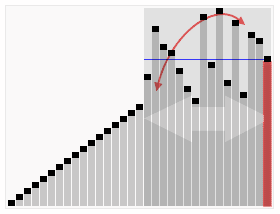
\includegraphics[width=0.8\linewidth]{sorting_quicksort_anim} \end{center}

Să observăm că există situații (de tipul \emph{cel mai rău caz}) în care
algoritmul Quicksort necesită \(\Omega(n)\)\footnote{A se vedea pagina
  de wikipedia
  \href{https://en.wikipedia.org/wiki/Big_O_notation}{Big\_O\_notation}}
operații de comparare. De exemplu să presupunem că lista de input este
\(S = \{x_1=n,x_2=n-1,\ldots,x_n=1\}\) și să presupunem că pentru
alegerea pivotului adoptăm regula ca acesta să fie primul element din
listă. Prin urmare primul pivot ales este \(n\) și algoritmul necesită
\(n-1\) comparații. În urma diviziunii, rezultă două subliste, una de
lungime \(0\) (care nu necesită nicio operație suplimentară) și una de
lungime \(n-1\) (ce elementele \(n-1, n-2, \ldots, 1\)). La pasul doi,
următorul pivot ales este \(n-1\) iar algoritmul necesită \(n-2\)
comparații și întoarce sublista cu elemente \(n-2, \ldots, 1\).
Continuând procedeul deducem că algoritmul Quicksort efectuează

\[
  (n-1) + (n-2) + \cdots + 1 = \frac{n(n-1)}{2} \quad \text{operații}.
\]

Din exemplul de mai sus, este clar că alegerea pivotului influențează
puternic numărul de operații pe care le efectuează algoritmul. O alegere
mai bună a pivotului ar consta în determinarea unui element, la fiecare
pas, care să împartă lista în două subliste cam de aceeași mărime
(\(\lceil n/2\rceil\) elemente).

Întrebarea care se pune este cum putem garanta că algoritmul alege un
pivot bun suficient de des ? O modalitate ar fi să alegem pivotul
aleator, de manieră uniformă între elementele disponibile. Această
abordare face ca algoritmul Quicksort să devină randomizat.

\begin{rmdexercise}
Să presupunem că ori de câte ori un pivot este ales pentru algoritmul
\emph{Quicksort randomizat}, acesta este ales independent și uniform din
mulțimea elementelor posibile. Arătați că numărul mediu de comparări ale
algoritmului este de \(2n\log(n)+O(n)\). Scrieți o funcție care
implementează algoritmul \emph{Quicksort randomizat} cu pivot ales
uniform.
\end{rmdexercise}

Fie \(y_1,\ldots, y_n\) elementele \(x_1,\ldots, x_n\) ordonate
crescător. Pentru \(i<j\), fie \(X_{ij}\) variabila aleatoare care ia
valoarea \(1\) dacă elementele \(y_i\) și \(y_j\) au fost comparate pe
parcursul rulării algoritmului și valoarea \(0\) altfel. Atunci numărul
total de comparări \(X\) satisface relația

\[
  X = \sum_{i = 1}^{n-1}\sum_{j = i+1}^{n}X_{ij}
\]

și din proprietatea de liniaritate a mediei

\[
  \mathbb{E}[X] = \mathbb{E}\left[\sum_{i = 1}^{n-1}\sum_{j = i+1}^{n}X_{ij}\right] = \sum_{i = 1}^{n-1}\sum_{j = i+1}^{n}\mathbb{E}[X_{ij}].
\]

Cum \(X_{ij}\) este o variabilă aleatoare de tip Bernoulli care ia doar
valoarea \(0\) și \(1\), \(\mathbb{E}[X_{ij}]=\mathbb{P}(X_{ij}=1)\)
prin urmare trebuie să determinăm probabilitatea ca elementele \(y_i\)
și \(y_j\) să fie comparate pe parcursul algoritmului. Să observăm că
elementele \(y_i\) și \(y_j\) sunt comparate dacă și numai dacă oricare
dintre cele două elemente sunt alese ca pivot din mulțimea
\(A_{ij} = \{y_i,y_{i+1},\ldots, y_j\}\). Acest lucru se datorează
faptului că dacă \(y_i\) (sau \(y_j\)) a fost primul pivot ales din
mulțimea \(A_{ij}\) atunci elementele \(y_i\) și \(y_j\) rămân în
aceeași sublistă, deci vor fi comparate ulterior. În mod similar, dacă
niciunul din elementele \(y_i\) și \(y_j\) nu este primul pivot ales din
mulțimea \(A_{ij}\) atunci cele două elemente vor face parte din
subliste separate și nu vor mai fi comparate.

Cum pivoții sunt aleși de manieră independentă și uniform din fiecare
sublistă de elemente, prima dată când un pivot este ales din mulțimea
\(A_{ij}\) acesta are aceeași șansă să fie oricare element. Prin urmare
probabilitatea ca \(y_i\) sau \(y_j\) să fie primul pivot ales este
\(\frac{2}{j-i+1}\). Astfel obținem

\begin{align*}
  \mathbb{E}[X] &= \sum_{i = 1}^{n-1}\sum_{j = i+1}^{n}\mathbb{E}[X_{ij}] = \sum_{i = 1}^{n-1}\sum_{j = i+1}^{n}\frac{2}{j-i+1} \\
         &= \sum_{i = 1}^{n-1}\sum_{k = 2}^{n-i+1}\frac{2}{k} = \sum_{k = 2}^{n}\sum_{i = 1}^{n+1-k}\frac{2}{k} \\
         &= \sum_{k = 2}^{n}(n+1-k)\frac{2}{k} = (2n+2)\sum_{k = 1}^{n}\frac{1}{k} - 4n.
\end{align*}

Prin urmare \(\mathbb{E}[X] = 2(n+1)H_n - 4n = 2n\log(n) + O(n)\) (am
folosit faptul că \(H_n = \log(n)+O(1)\)\footnote{A se vedea pagina de
  wikipedia
  \href{https://en.wikipedia.org/wiki/Harmonic_number}{armonic\_number}}).

Următorul cod implementează algoritmul \emph{Quicksort randomizat}:

\begin{Shaded}
\begin{Highlighting}[]
\NormalTok{quickSort <-}\StringTok{ }\ControlFlowTok{function}\NormalTok{(vect) \{}
  \CommentTok{# Args:}
  \CommentTok{#  vect: Vector numeric}
  
  \CommentTok{# daca lungimea este <= 1 stop}
  \ControlFlowTok{if}\NormalTok{ (}\KeywordTok{length}\NormalTok{(vect) }\OperatorTok{<=}\StringTok{ }\DecValTok{1}\NormalTok{) \{}
    \KeywordTok{return}\NormalTok{(vect)}
\NormalTok{  \}}
  
  \CommentTok{# alege pivotul}
\NormalTok{  ide =}\StringTok{ }\KeywordTok{sample}\NormalTok{(}\DecValTok{1}\OperatorTok{:}\KeywordTok{length}\NormalTok{(vect),}\DecValTok{1}\NormalTok{)}
\NormalTok{  element =}\StringTok{ }\NormalTok{vect[ide]}
\NormalTok{  partition =}\StringTok{ }\NormalTok{vect[}\OperatorTok{-}\NormalTok{ide]}
  
  \CommentTok{# Imparte elementele in doua subliste (< pivot si >= pivot)}
\NormalTok{  v1 =}\StringTok{ }\NormalTok{partition[partition }\OperatorTok{<}\StringTok{ }\NormalTok{element]}
\NormalTok{  v2 =}\StringTok{ }\NormalTok{partition[partition }\OperatorTok{>=}\StringTok{ }\NormalTok{element]}
  
  \CommentTok{# Aplica recursiv algoritmul}
\NormalTok{  v1 =}\StringTok{ }\KeywordTok{quickSort}\NormalTok{(v1)}
\NormalTok{  v2 =}\StringTok{ }\KeywordTok{quickSort}\NormalTok{(v2)}
  \KeywordTok{return}\NormalTok{(}\KeywordTok{c}\NormalTok{(v1, element, v2))}
\NormalTok{\}}

\NormalTok{n =}\StringTok{ }\DecValTok{25}
\NormalTok{S =}\StringTok{ }\KeywordTok{sample}\NormalTok{(}\DecValTok{1}\OperatorTok{:}\NormalTok{n, n, }\DataTypeTok{replace =} \OtherTok{FALSE}\NormalTok{)}
\CommentTok{# lista neordonata}
\NormalTok{S}
\NormalTok{ [}\DecValTok{1}\NormalTok{] }\DecValTok{20}  \DecValTok{8} \DecValTok{13}  \DecValTok{5} \DecValTok{15}  \DecValTok{9} \DecValTok{22} \DecValTok{11}  \DecValTok{4} \DecValTok{18} \DecValTok{19}  \DecValTok{6}  \DecValTok{2} \DecValTok{14} \DecValTok{21} \DecValTok{23}  \DecValTok{3} \DecValTok{16} \DecValTok{24} \DecValTok{17} \DecValTok{12} \DecValTok{25}  \DecValTok{7}
\NormalTok{[}\DecValTok{24}\NormalTok{]  }\DecValTok{1} \DecValTok{10}
\CommentTok{# lista ordonata}
\KeywordTok{quickSort}\NormalTok{(S)}
\NormalTok{ [}\DecValTok{1}\NormalTok{]  }\DecValTok{1}  \DecValTok{2}  \DecValTok{3}  \DecValTok{4}  \DecValTok{5}  \DecValTok{6}  \DecValTok{7}  \DecValTok{8}  \DecValTok{9} \DecValTok{10} \DecValTok{11} \DecValTok{12} \DecValTok{13} \DecValTok{14} \DecValTok{15} \DecValTok{16} \DecValTok{17} \DecValTok{18} \DecValTok{19} \DecValTok{20} \DecValTok{21} \DecValTok{22} \DecValTok{23}
\NormalTok{[}\DecValTok{24}\NormalTok{] }\DecValTok{24} \DecValTok{25}
\end{Highlighting}
\end{Shaded}

Numărul mediu de comparații pe care le efectuează algoritmul
\emph{Quicksort randomizat}, versiunea empirică versus cea teoretică de
mai sus, este ilustrat în figura următoare:

\begin{center}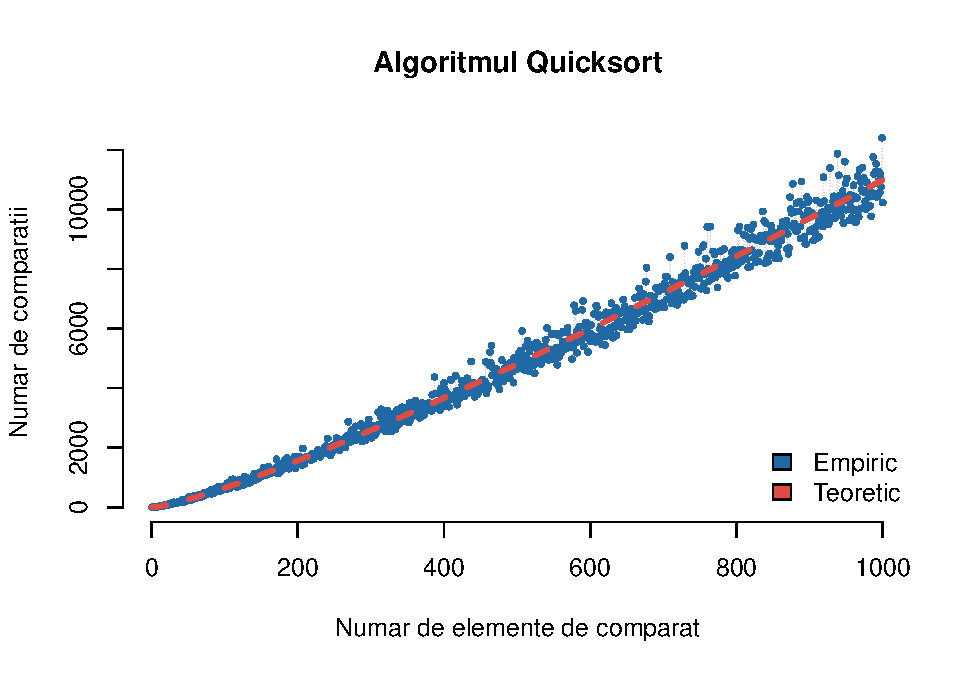
\includegraphics[width=0.8\linewidth]{Lab5_files/figure-latex/unnamed-chunk-7-1} \end{center}

Pentru a reproduce figura de mai sus trebuie modificat codul funcției
\texttt{quickSort} pentru a returna și numărul de comparații efectuate:

\begin{Shaded}
\begin{Highlighting}[]
\NormalTok{countQuickSort <-}\StringTok{ }\ControlFlowTok{function}\NormalTok{(vect) \{}
  \CommentTok{# Args:}
  \CommentTok{#  vect: Vector numeric}
  
  \CommentTok{# daca lungimea este <= 1 stop}
  \ControlFlowTok{if}\NormalTok{ (}\KeywordTok{length}\NormalTok{(vect) }\OperatorTok{<=}\StringTok{ }\DecValTok{1}\NormalTok{) \{}
    \KeywordTok{return}\NormalTok{(vect)}
\NormalTok{  \}}
  
  \CommentTok{# intoarce numarul de comaparatii efectuate}
\NormalTok{  count <<-}\StringTok{ }\NormalTok{count }\OperatorTok{+}\StringTok{ }\KeywordTok{length}\NormalTok{(vect) }\OperatorTok{-}\StringTok{ }\DecValTok{1} 
  
  \CommentTok{# alege pivotul}
\NormalTok{  ide =}\StringTok{ }\KeywordTok{sample}\NormalTok{(}\DecValTok{1}\OperatorTok{:}\KeywordTok{length}\NormalTok{(vect),}\DecValTok{1}\NormalTok{)}
\NormalTok{  element =}\StringTok{ }\NormalTok{vect[ide]}
\NormalTok{  partition =}\StringTok{ }\NormalTok{vect[}\OperatorTok{-}\NormalTok{ide]}
  
  \CommentTok{# Imparte elementele in doua subliste (< pivot si >= pivot)}
\NormalTok{  v1 =}\StringTok{ }\NormalTok{partition[partition }\OperatorTok{<}\StringTok{ }\NormalTok{element]}
\NormalTok{  v2 =}\StringTok{ }\NormalTok{partition[partition }\OperatorTok{>=}\StringTok{ }\NormalTok{element]}
  
  \CommentTok{# Aplica recursiv algoritmul}
\NormalTok{  v1 =}\StringTok{ }\KeywordTok{countQuickSort}\NormalTok{(v1)}
\NormalTok{  v2 =}\StringTok{ }\KeywordTok{countQuickSort}\NormalTok{(v2)}
  \KeywordTok{return}\NormalTok{(}\KeywordTok{c}\NormalTok{(v1, element, v2))}
\NormalTok{\}}

\NormalTok{N =}\StringTok{ }\DecValTok{1000}
\NormalTok{y =}\StringTok{ }\KeywordTok{rep}\NormalTok{(}\DecValTok{0}\NormalTok{, N)}

\ControlFlowTok{for}\NormalTok{ (i }\ControlFlowTok{in} \DecValTok{1}\OperatorTok{:}\NormalTok{N)\{}
\NormalTok{  S =}\StringTok{ }\KeywordTok{sample}\NormalTok{(}\DecValTok{1}\OperatorTok{:}\NormalTok{i, i, }\DataTypeTok{replace =} \OtherTok{FALSE}\NormalTok{)}
  
\NormalTok{  count =}\StringTok{ }\DecValTok{0}
\NormalTok{  S_sort =}\StringTok{ }\KeywordTok{countQuickSort}\NormalTok{(S)}
  
\NormalTok{  y[i] =}\StringTok{ }\NormalTok{count}
\NormalTok{\}}
\end{Highlighting}
\end{Shaded}

iar graficul se realizează apelând următorul cod:

\begin{Shaded}
\begin{Highlighting}[]
\CommentTok{# Graficul}
\KeywordTok{plot}\NormalTok{(}\DecValTok{1}\OperatorTok{:}\NormalTok{N, y, }\DataTypeTok{type =} \StringTok{"l"}\NormalTok{, }
     \DataTypeTok{col =} \StringTok{"grey80"}\NormalTok{,}
     \DataTypeTok{bty =} \StringTok{"n"}\NormalTok{, }
     \DataTypeTok{main =} \StringTok{"Algoritmul Quicksort"}\NormalTok{,}
     \DataTypeTok{xlab =} \StringTok{"Numar de elemente de comparat"}\NormalTok{,}
     \DataTypeTok{ylab =} \StringTok{"Numar de comparatii"}\NormalTok{,}
     \DataTypeTok{lty =} \DecValTok{3}\NormalTok{,}
     \DataTypeTok{lwd =} \FloatTok{0.5}\NormalTok{)}
\KeywordTok{points}\NormalTok{(}\DecValTok{1}\OperatorTok{:}\NormalTok{N, y, }
       \DataTypeTok{col =} \StringTok{"royalblue"}\NormalTok{, }
       \DataTypeTok{pch =} \DecValTok{16}\NormalTok{,}
       \DataTypeTok{cex =} \FloatTok{0.6}\NormalTok{)}
\KeywordTok{lines}\NormalTok{(}\DecValTok{1}\OperatorTok{:}\NormalTok{N, theo_T, }\DataTypeTok{col =} \StringTok{"brown3"}\NormalTok{, }\DataTypeTok{lwd =} \DecValTok{3}\NormalTok{, }\DataTypeTok{lty =} \DecValTok{2}\NormalTok{)}
\KeywordTok{legend}\NormalTok{(}\StringTok{'bottomright'}\NormalTok{, }
       \DataTypeTok{legend =} \KeywordTok{c}\NormalTok{(}\StringTok{"Empiric"}\NormalTok{, }\StringTok{"Teoretic"}\NormalTok{), }
       \DataTypeTok{fill =} \KeywordTok{c}\NormalTok{(}\StringTok{"royalblue"}\NormalTok{, }\StringTok{"brown3"}\NormalTok{),}
       \DataTypeTok{bty =} \StringTok{"n"}\NormalTok{)}
\end{Highlighting}
\end{Shaded}


\end{document}
